\documentclass[12pt]{article}
 
\title{Attitude control of miniature quadrotor}
\author{Nestor A Eduartes}

\usepackage[top=1in, bottom=1.25in, left=1.25in, right=1.25in]{geometry}
\usepackage{amsmath}
\usepackage{graphicx}

\begin{document}
 
\maketitle
 
\begin{abstract}
Two control schemes are evaluated for the attitude control of a hovering quad rotor based on the non linear lagrangian dynamic model. The system model is developed based on a set of parameter for a theoretical quad rotor. Attitude control is performed using a set of independent pole placement state feedback controlled based on a linearized decoupled model simplification. A second controller is designed using an optimal linear quadratic state feedback regulator, based on a linear model. The performance of both controllers are assessed by the response to small disturbances around the hovering state.
\end{abstract}

\section{Introduction}
The quadrotor concept is particularly interesting in the research of Unmanned Aerial Vehicles due to its simple architecture and flexibility for control compared to other helicopter designs. The four propeller design allows to achieve a complete control of the attitude and position of the structure using simple mechanical actuators. The quadrotor platform has been subject to broad research given the ease of construction, high  maneuverability, and ability to hover \cite{Cabe14}.

The quad rotor architecture achieves its lift through two pairs of propellers installed in cross configuration. The pair of propellers (1,3) and (2,4) turn in opposite directions by the action of four electric motors. By varying the rotor speed of each motor, a change in the lift torque is achieved. The total thrust of the structure is controlled by jointly modifying the speed of the four propellers. 

The orientation of the quadrotor depends on the relationship of the speed of the four propellers. A difference between the rotor speed of propellers 2 and 4 generates a rotation about the roll direction and a motion in the y-axis. Conversely, a difference between the rotor speed of propellers 1 and 3 generates a rotation about the pitch direction and a motion in the x-axis. Finally, the difference in the torque generated by each pair of propellers generates a yaw rotation.

It is clear that a precise control of the four motors is required to achieve a stable operation and control of the position and attitude of the quadrotor structure. In the following sections the dynamic model of the quadrotor is presented, and a brief survey on control strategies is exposed. Two classical strategies are developed and compared.

\section{Quadrotor dynamic model}
\label{sec:dynamics}
The dynamic model for the quadrotor is taken from \cite{Boua04}. This dynamic model is particularly interesting since it includes the gyroscopic effects to which the structure is subject due to the action of the propeller's rotation. This aspects are particularly interesting since the dynamics of the model will be simulated to assess the control strategies.

The dynamic of the quadrotor can be described using its coordinates on an earth fixed frame, together with the orientation of the structure in space. This model representation yields 12 states comprising: 3 position coordinates, and their rates of change; and 3 Euler angles, and ther rates of changes. The Euler angles are defined by the following convention: \emph{roll} $\phi$, as the rotation around the x-axis; \emph{pitch} $\theta$, as the rotation around the y-axis; and \emph{yaw} $\psi$, as the rotation around the z-axis. The configuration of the quadrotor is shown in Figure X.

The dynamic model is derived using Euler-Lagrange mecanical formulation under the following assumptions \cite{Boua04}:

\begin{itemize}
\item The structure is assumed as rigid.
\item The structure is assumed as symmetrical.
\item The body fixed frame is defined in the center of mass of the body.
\item The propellers are assumed rigid.
\item The thrust and drag of the propellers are proportional to the square of the propeller speed.
\end{itemize}

This assumptions allows us to represent the object by its inertia matrix, and a point mass at the center of gravity. The assumption of symmetry allows to assume that the inertia matrix is diagonal, further simplifying the model. Since the objective of this project is to evaluate the control strategies for the attitude control of the quadrotor, the translational dynamics are not considered. 

The model for the attitude dynamics of the quadrotor are given by:

\begin{equation}
  \label{eq:dynamics}
  \begin{split}
    \ddot{\phi} &= \dot{\theta} \dot{\psi} \left ( \frac{I_y-I_z}{I_x} \right ) - \frac{J}{I_x} \dot{\theta} \Omega + \frac{l}{I_x} U_1 \\
    \ddot{\theta} &= \dot{\phi} \dot{\psi} \left ( \frac{I_z-I_x}{I_y} \right ) + \frac{J}{I_y} \dot{\phi} \Omega + \frac{l}{I_y} U_2 \\
    \ddot{\psi} &= \dot{\phi} \dot{\theta} \left ( \frac{I_x-I_y}{I_z} \right ) + \frac{1}{I_z} U_3
  \end{split}
\end{equation}

The control inputs are related to the rotor speeds are given by:

\begin{equation}
  \label{eq:inputs}
  \begin{split}
  U_1 &= b \left (\Omega^2_4 - \Omega^2_2 \right ) \\
  U_2 &= b \left (\Omega^2_3 - \Omega^2_1 \right ) \\
  U_3 &= d \left (\Omega^2_1 + \Omega^2_3 - \Omega^2_2 - \Omega^2_4 \right ) \\
  \Omega &= \Omega^2_1 + \Omega^2_2 + \Omega^2_3 + \Omega^2_4
  \end{split}
\end{equation}

Where each constant for our case of study are shown in Table~\ref{tab:parameters}. These parameters are taken from \cite{Merh14}:

\begin{table}
  \begin{center}
    \caption{Quadrotor parameters}\label{tab:parameters}
    \begin{tabular}{rlr}
      \hline
      Parameter & Definition & Value \\
      \hline                  
      $I_x$ & x-axis inertia & $8.10 \times {10}^{-3}$\\
      $I_y$ & y-axis inertia & $8.10 \times {10}^{-3}$\\
      $I_z$ & z-axis inertia & $1.42 \times {10}^{-2}$ \\
      $J$ & propeller inertia & $1.04 \times {10}^{-4}$ \\
      $b$ & thrust factor & $ 5.42 \times {10}^{-5}$ \\
      $d$ & drag factor & $ 1.10 \times{10}^{-6}$ \\
      $l$ & arm length & $0.24$ \\
      \hline
    \end{tabular}
  \end{center}
\end{table}

\section{Control architecture}
One common control architecture comprises a hierarchical control of the quadrotor dynamics. This hierarchical scheme comprises an inner control loop, consisting of the attitude control of the quadrotor, together with an outer loop, controlling the translational dynamics of the quadrotor \cite{Raff10}. This architecture allows a greater flexibility in the development of the control modules. This scheme allows the manual operation of the quadrotor by an operator, subsitituting the outer control loop. The outer loop reference signals can be generated from a mission control system, responsible of computing the desired trajectory. The propossed architecture is shown in Figure \ref{fig:control}.

This hierarchical structure allows us to work on the attitude control in an independent manner without a loss in generality.

\begin{figure}
  \centering
  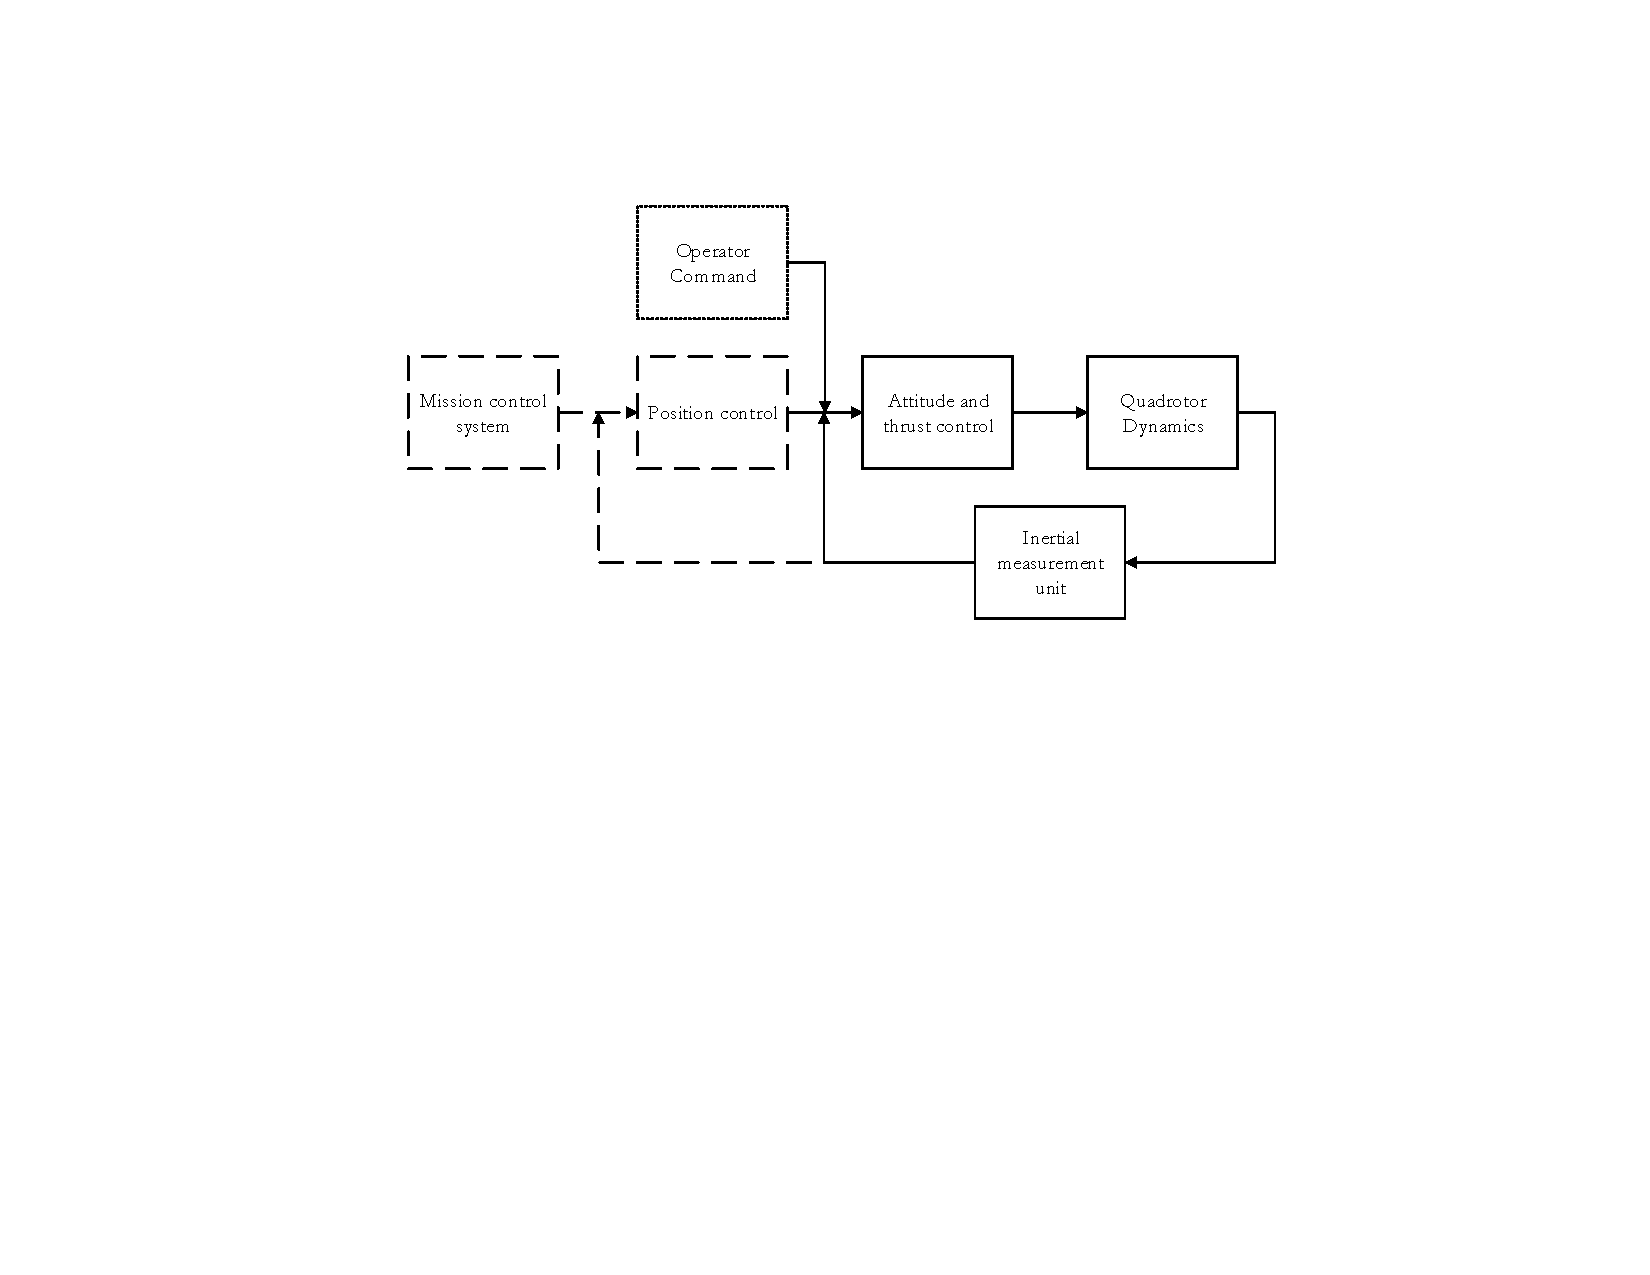
\includegraphics{control.pdf}
  \caption{Control architecture.}
  \label{fig:control}
\end{figure}

\subsection{Model Linearization}
\label{sec:linearization}
The linear system for (\ref{eq:dynamics}) can be calculated through the first-order Taylor series expansion around $\left (\bar{x},\bar{u} \right )$, such that this is an equilibrium point.

\begin{equation}
  \begin{split}
    \dot{x}(t) &= f(x(t)) + g(u(t)) \\
    \Delta x(t) &:= x(t) - \bar{x} \\
    \Delta u(t) &:= u(t) - \bar{u} \\
    \bar{\dot{x}}(t) &= f(\bar{x}) + g(\bar{u}) = 0
  \end{split}
\end{equation}

Then the linear model around the equilibrium point can be calculated using the first-order Taylor series expansion. Where $\tilde{A}$ and $\tilde{B}$ are the Jacobians of the nonlinear functions $f(x)$ and $g(u)$, and $\epsilon (t)$ is the error due to the terms of second order and higher.

\begin{equation}
  \begin{split}
    \label{eq:linearization}
    \Delta\dot{x}(t) &\approx  \tilde{A} \, \Delta x(t) + \tilde{B} \, \Delta u(t) + \epsilon (t) \\
    \tilde{A} &= \left. \frac{ \partial f(x)} {\partial x} \right|_{\begin{smallmatrix} x = \bar{x} \\ u = \bar{u} \end{smallmatrix}} = \begin{bmatrix}
    \frac{\partial f_1(\mathbf{x})}{\partial x_1} & \cdots & \frac{\partial f_1(\mathbf{x})}{\partial x_n} \\
    \vdots & \ddots & \vdots \\
    \frac{\partial f_n(\mathbf{x})}{\partial x_1} & \cdots & \frac{\partial f_n(\mathbf{x})}{\partial x_n}
    \end{bmatrix} \\
    \tilde{B} &= \left. \frac{\partial g(u)} {\partial u} \right|_{u = \bar{u}} = \begin{bmatrix}
    \frac{\partial g_1(\mathbf{x})}{\partial x_1} & \cdots & \frac{\partial g_1(\mathbf{x})}{\partial x_m} \\
    \vdots & \ddots & \vdots \\
    \frac{\partial g_n(\mathbf{x})}{\partial x_1} & \cdots & \frac{\partial g_n(\mathbf{x})}{\partial x_m}
    \end{bmatrix} \\
  \end{split}
\end{equation}

\subsection{Quadrotor linearized model}

The quadrotor has an equilibrium point at hover. That is $ x(t) = 0 $. By performing the linearization process described in Section \ref{sec:linearization}, we can find a description of the quadrotor dynamics near the hover position as:

\begin{equation}
  \begin{split}
    \Omega_o = \sqrt{\frac{mg}{4b}} = \sqrt{\frac{\left( 1 kg \right) \times \left( 9.8m/s^2 \right)}{4 \times \left (2.017\times 10^{-5} \right )}} = 212.61 rev/sec
  \end{split}
\end{equation}

$$ \tilde{A} = 
{\left. \begin{bmatrix}
0 & 1 & 0 & 0 & 0 & 0 \\ 
0 & 0 & 0 & \dot{\psi} \left (\frac{I_y - I_z}{I_x} \right ) - \frac{J}{I_x} \Omega & 0 & \dot{\theta} \left (\frac{I_y - I_z}{I_x} \right ) \\ 
0 & 0 & 0 & 1 & 0 & 0 \\ 
0 & \dot{\psi} \left (\frac{I_z - I_x}{I_y} \right ) + \frac{J}{I_y} \Omega & 0 & 0 & 0 & \dot{\phi} \left (\frac{I_z - I_x}{I_y} \right ) \\ 
0 & 0 & 0 & 0 & 0 & 1 \\ 
0 & \dot{\theta} \left (\frac{I_x - I_y}{I_z} \right ) & 0 & \dot{\phi} \left (\frac{I_x - I_y}{I_z} \right ) & 0 & 0
\end{bmatrix} \right |}_{\begin{smallmatrix} x = 0 \\ u = \bar{u} \end{smallmatrix}} $$

\begin{equation}
\tilde{A} = 
\begin{bmatrix}
0 & 1 & 0 & 0 & 0 & 0 \\ 
0 & 0 & 0 & -\frac{J}{I_x} \Omega_o & 0 & 0 \\ 
0 & 0 & 0 & 1 & 0 & 0 \\ 
0 & \frac{J}{I_y} \Omega_o & 0 & 0 & 0 & 0 \\ 
0 & 0 & 0 & 0 & 0 & 1 \\ 
0 & 0 & 0 & 0 & 0 & 0
\end{bmatrix}
\end{equation}

\begin{equation}
\tilde{B} = 
\begin{bmatrix}
0 & 0 & 0 \\ 
\frac{l}{I_x} & 0 & 0 \\
0 & 0 & 0 \\ 
0 & \frac{l}{I_y} & 0 \\
0 & 0 & 0 \\ 
0 & 0 & \frac{l}{I_z}
\end{bmatrix}
\end{equation}

The linearization of the control input given the rotor speed can be found in an analogous way.

\begin{equation}
  \label{eq:controls}
  \begin{bmatrix}
  U_1 \\ U_2 \\ U_3 \\ \Omega
  \end{bmatrix} = \mathbf{M}
  \begin{bmatrix}
  \Omega_1 \\ \Omega_2 \\ \Omega_3 \\ \Omega_4
  \end{bmatrix},\quad \mathbf{M} = 2\Omega_o
  \begin{bmatrix}
  0 & -b & 0 & b \\ 
  -b & 0 & b & 0 \\ 
  d & -d & d & -d \\
  1 & 1 & 1 & 1
  \end{bmatrix}
\end{equation}

By including the constrain $ \Omega = 0 $, we can assure that the attitude control inputs will not change the total thrust on the quadrotor. Under this assumption, then $ \mathbf{M} $ is invertible, and we can construct the mapping for the speed control given the desired control input vector $ \begin{bmatrix} U_1  & U_2 & U_3 & 0\end{bmatrix}^\mathrm{T} $.

\begin{equation}
    \begin{bmatrix}
    \Omega_1 \\ \Omega_2 \\ \Omega_3 \\ \Omega_4
    \end{bmatrix} = 
    \mathbf{M}^{-1} \begin{bmatrix} U_1 \\ U_2 \\ U_3 \\ 0 \end{bmatrix},\quad
    \mathbf{M}^{-1} = \frac{1}{2 \Omega_o}
    \begin{bmatrix}
    0 & -\frac{1}{2b} & \frac{1}{4d} & \frac{1}{4} \\ 
    -\frac{1}{2b} & 0 & -\frac{1}{4d} & \frac{1}{4} \\ 
    0 & \frac{1}{2b} & \frac{1}{4d} & \frac{1}{4} \\
    \frac{1}{2b} & 0 & -\frac{1}{4d} & \frac{1}{4}
    \end{bmatrix}
\end{equation}

\section{Controller Design}

Two different linear approaches are evaluated in the following sections. These are a State Feedback Controller design by pole placement technique, and a Linear Quadratic Optimal Controller.

\subsection{State Feedback Controller}
\label{sec:state-feedback}

The state feedback controller is designed using the linearized state space representation of the system. To generate the feedback control law $K$ for the closed loop system, the key performance indexes for the dynamic response is propossed. The objective of this controller is to replicate the results found in \cite{Boua04} for the PID controller design. Therefore, the key performance indexes are evaluated from the results found for the PID controller. The identified key performance indexes are shown in Table~\ref{tab:KPI}.

\begin{table}
  \begin{center}
    \caption{Key performance index}
    \label{tab:KPI}
    \begin{tabular}{rlr}
      \hline
      Symbol & Index & Value \\
      \hline                  
      $T_s$ & Settling time & $1$ [sec]\\
      $\%OS$ & Percentage Overshot & $10\%$\\
      \hline
    \end{tabular}
  \end{center}
\end{table}

The linearized system found in Section \ref{sec:linear} is a coupled MIMO system. This poses certain difficulties for the controller design. The approach for this case, is to consider the cross-coupling terms as a disturbance. When the cross-coupling terms are excluded, the system dynamics reduces to 3 SISO systems. Therefore, the design consists of three parallel state feedback controllers. Each of the 

\begin{equation}
\dot{\mathbf{x}} = \mathbf{A} \mathbf{x} + \mathbf{B} \mathbf{u}
\end{equation}

\begin{equation}
\mathbf{A} = diag\begin{bmatrix} \mathbf{A}_\theta & \mathbf{A}_\theta & \mathbf{A}_\psi \end{bmatrix}
\end{equation}

\begin{equation}
\mathbf{B} = diag\begin{bmatrix} \mathbf{B}_\theta & \mathbf{B}_\theta & \mathbf{B}_\psi \end{bmatrix}
\end{equation}

\begin{equation}
\mathbf{x} = \begin{bmatrix} \mathbf{x}_\theta & \mathbf{x}_\theta & \mathbf{x}_\psi \end{bmatrix}
\end{equation}

\begin{equation}
\mathbf{u} = \begin{bmatrix} u_1 & u_2 & u_3 \end{bmatrix}
\end{equation}

\section{Linear Quadratic Regulator}

\section{System simulation}
A Simulink block performing the nonlinear dynamic model described in section~\ref{sec:dynamics} was created. Two control strategies were performed to control de dynamics of the quadrotor. Figure~\ref{fig:simulink} shows the State Feedback Regulator designed in section~\ref{sec:state-feedback}.

\begin{figure}
  \centering
  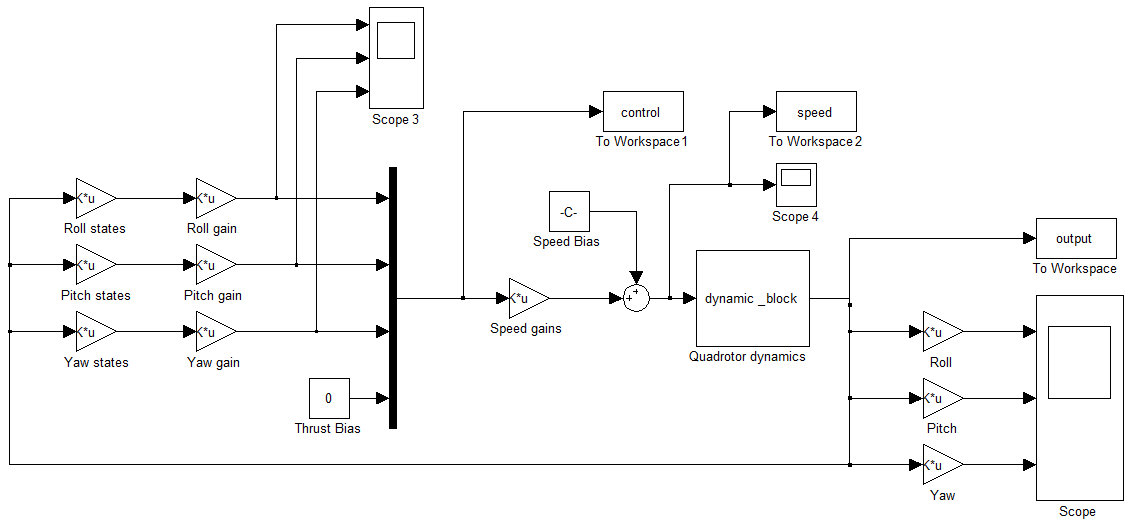
\includegraphics[width=0.7\textwidth]{Simulink.png}
  \caption{Simulink model.}
  \label{fig:model}
\end{figure}

\section{Results}

\subsection{State feedback controller}

\begin{figure}
  \centering
  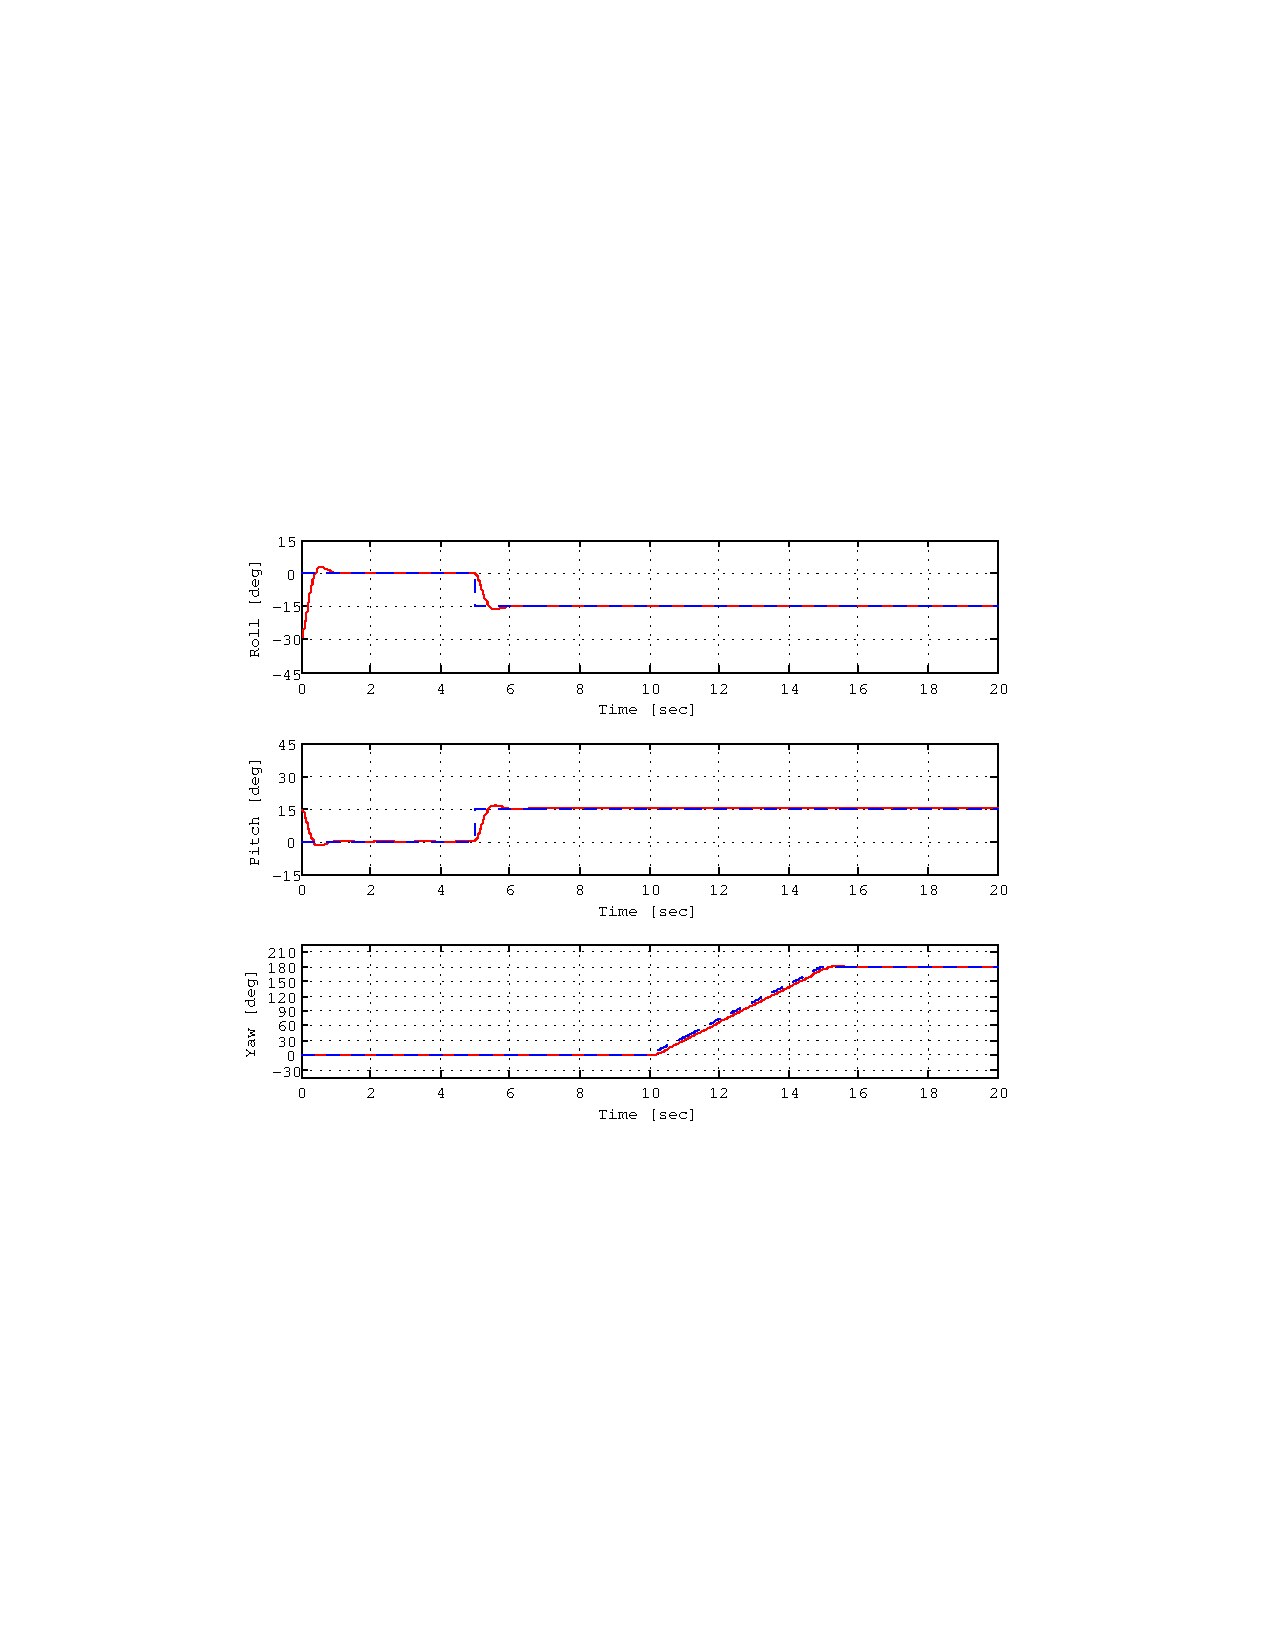
\includegraphics{state-feedback.pdf}
  \caption{System response for initial states $\mathbf{x} = \begin{bmatrix} 1.2 & -0.1 & 0.65 & 0.1 & 0.5 & 0 \end{bmatrix}^\mathrm{T} $.}
  \label{fig:res-sf}
\end{figure}

\subsection{Linear Quadratic Regulator Controller}

\begin{figure}
  \centering
  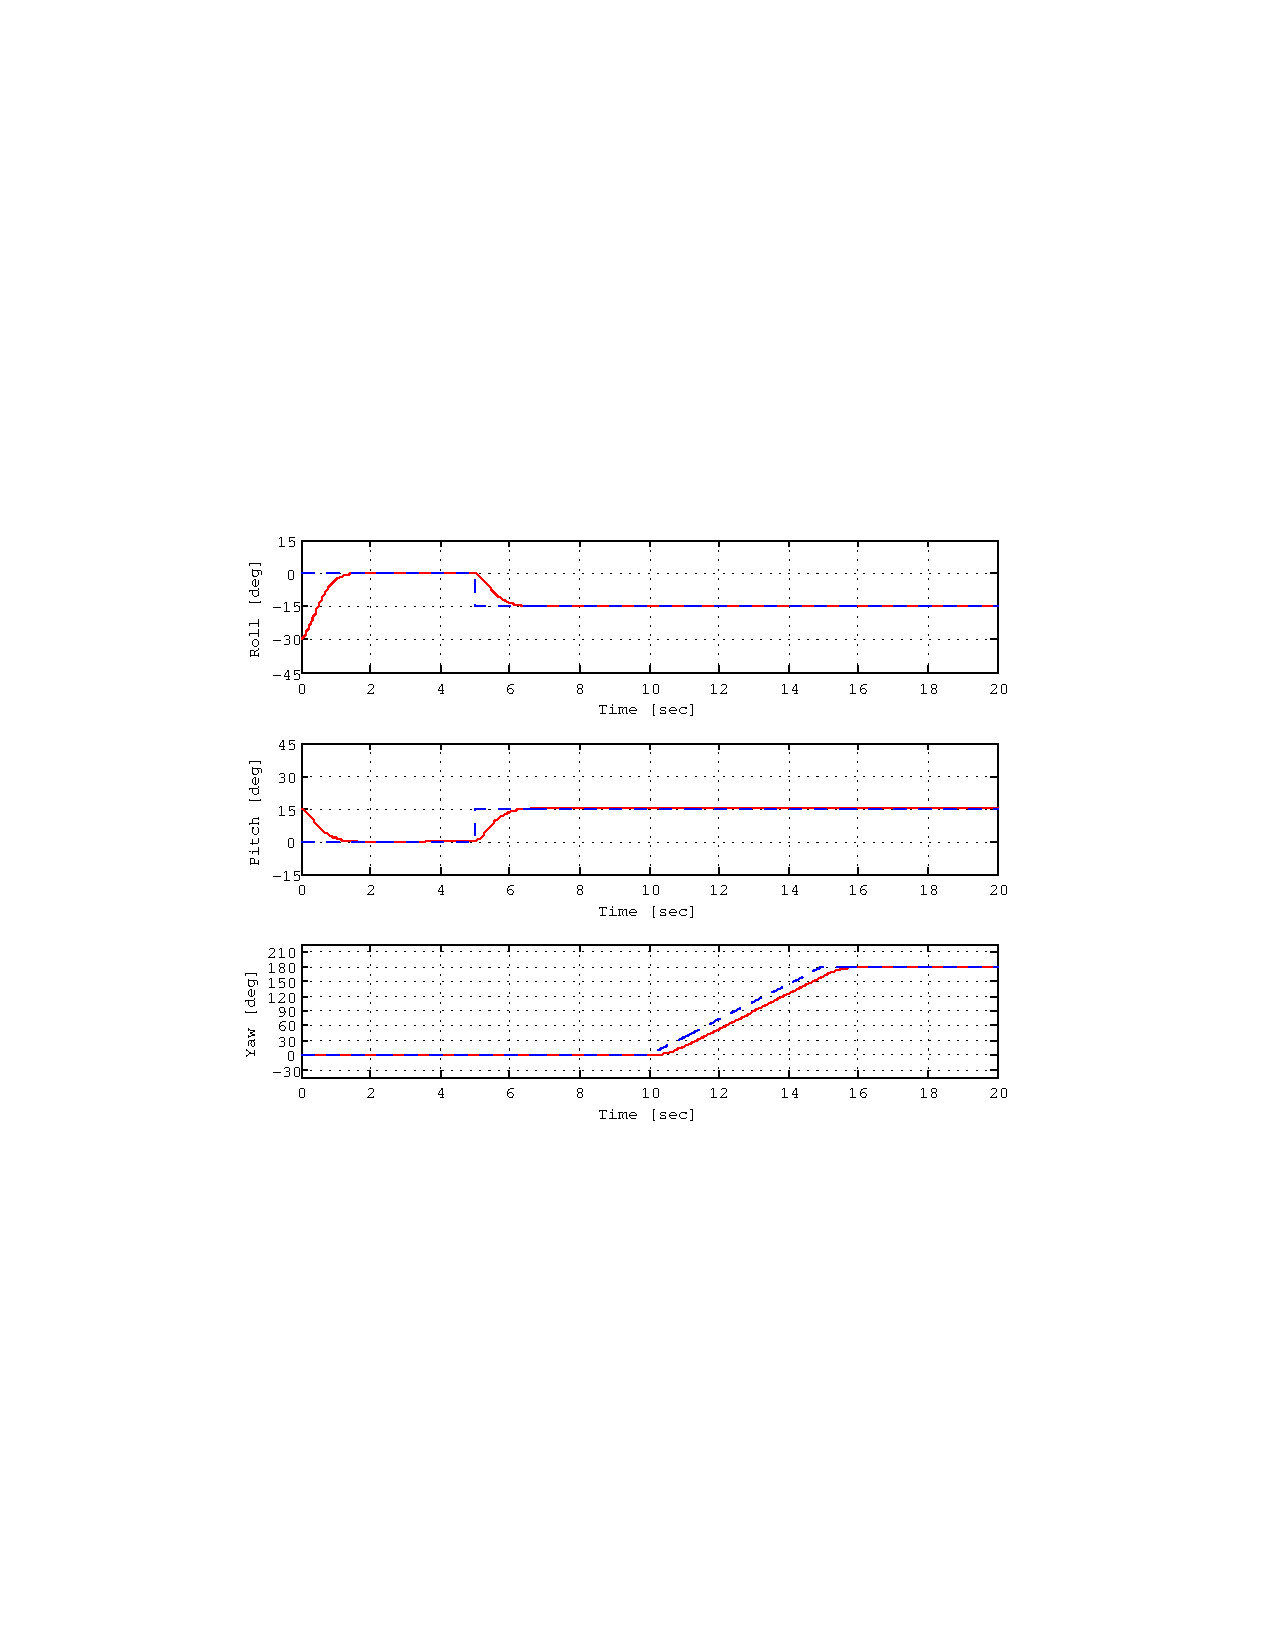
\includegraphics{lqg.pdf}
  \caption{System response for initial states $\mathbf{x} = \begin{bmatrix} 1.2 & -0.1 & 0.65 & 0.1 & 0.5 & 0 \end{bmatrix}^\mathrm{T} $.}
  \label{fig:control}
\end{figure}

\begin{table}
  \begin{center}
    \caption{Key performance index}
    \label{tab:KPI}
    \begin{tabular}{rlr}
      \hline
      Symbol & Index & Value \\
      \hline                  
      $T_s$ & Settling time & $1$ [sec]\\
      $\%OS$ & Percentage Overshot & $10\%$\\
      \hline
    \end{tabular}
  \end{center}
\end{table}


\section{Appendix A: Systems matrixes}


 
\begin{thebibliography}{100} % 100 is a random guess of the total number of
\bibitem{Merh14} Merheb A., Noura H., and Bateman F., (2014)
``Active fault tolerant control of quadrotor UAV using Sliding Mode Control"
\emph{Proceedings of the International Conference on Unmanned Aircraft Systems (ICUAS)},
(pp. 156-166).

\bibitem{Boua04} Bouabdallah S., Noth A., and Siegwart R., (2004) 
``PID vs LQ Control Techniques Applied to an Indoor Micro Quadrotor". 
\emph{Proceedings of the International Conference of Intelligent Robots and Systems}, 
(pp. 2451-2456).

\bibitem{Cabe14} Cabecinhas D., Cunha R., and Silvestre C., (2014),
``A nonlinear quadrotor trajectory tracking controller with disturbance rejection".
\emph{Journal Control Engineering Practice}, Volume 26, (pp. 1–10).

\bibitem{Raff10} Raffo G., Ortega M., and Rubio F., (2010)
``An integral predictive/nonlinear $\mathcal{H} _\infty$ control structure for a quadrotor helicopter"
\emph{Journal Automatica}, Volume 46, (pp. 29-39)
\end{thebibliography}

\end{document}